
% Default to the notebook output style

    


% Inherit from the specified cell style.




    
\documentclass[11pt]{article}

    
    
    \usepackage[T1]{fontenc}
    % Nicer default font (+ math font) than Computer Modern for most use cases
    \usepackage{mathpazo}

    % Basic figure setup, for now with no caption control since it's done
    % automatically by Pandoc (which extracts ![](path) syntax from Markdown).
    \usepackage{graphicx}
    % We will generate all images so they have a width \maxwidth. This means
    % that they will get their normal width if they fit onto the page, but
    % are scaled down if they would overflow the margins.
    \makeatletter
    \def\maxwidth{\ifdim\Gin@nat@width>\linewidth\linewidth
    \else\Gin@nat@width\fi}
    \makeatother
    \let\Oldincludegraphics\includegraphics
    % Set max figure width to be 80% of text width, for now hardcoded.
    \renewcommand{\includegraphics}[1]{\Oldincludegraphics[width=.8\maxwidth]{#1}}
    % Ensure that by default, figures have no caption (until we provide a
    % proper Figure object with a Caption API and a way to capture that
    % in the conversion process - todo).
    \usepackage{caption}
    \DeclareCaptionLabelFormat{nolabel}{}
    \captionsetup{labelformat=nolabel}

    \usepackage{adjustbox} % Used to constrain images to a maximum size 
    \usepackage{xcolor} % Allow colors to be defined
    \usepackage{enumerate} % Needed for markdown enumerations to work
    \usepackage{geometry} % Used to adjust the document margins
    \usepackage{amsmath} % Equations
    \usepackage{amssymb} % Equations
    \usepackage{textcomp} % defines textquotesingle
    % Hack from http://tex.stackexchange.com/a/47451/13684:
    \AtBeginDocument{%
        \def\PYZsq{\textquotesingle}% Upright quotes in Pygmentized code
    }
    \usepackage{upquote} % Upright quotes for verbatim code
    \usepackage{eurosym} % defines \euro
    \usepackage[mathletters]{ucs} % Extended unicode (utf-8) support
    \usepackage[utf8x]{inputenc} % Allow utf-8 characters in the tex document
    \usepackage{fancyvrb} % verbatim replacement that allows latex
    \usepackage{grffile} % extends the file name processing of package graphics 
                         % to support a larger range 
    % The hyperref package gives us a pdf with properly built
    % internal navigation ('pdf bookmarks' for the table of contents,
    % internal cross-reference links, web links for URLs, etc.)
    \usepackage{hyperref}
    \usepackage{longtable} % longtable support required by pandoc >1.10
    \usepackage{booktabs}  % table support for pandoc > 1.12.2
    \usepackage[inline]{enumitem} % IRkernel/repr support (it uses the enumerate* environment)
    \usepackage[normalem]{ulem} % ulem is needed to support strikethroughs (\sout)
                                % normalem makes italics be italics, not underlines
    

    
    
    % Colors for the hyperref package
    \definecolor{urlcolor}{rgb}{0,.145,.698}
    \definecolor{linkcolor}{rgb}{.71,0.21,0.01}
    \definecolor{citecolor}{rgb}{.12,.54,.11}

    % ANSI colors
    \definecolor{ansi-black}{HTML}{3E424D}
    \definecolor{ansi-black-intense}{HTML}{282C36}
    \definecolor{ansi-red}{HTML}{E75C58}
    \definecolor{ansi-red-intense}{HTML}{B22B31}
    \definecolor{ansi-green}{HTML}{00A250}
    \definecolor{ansi-green-intense}{HTML}{007427}
    \definecolor{ansi-yellow}{HTML}{DDB62B}
    \definecolor{ansi-yellow-intense}{HTML}{B27D12}
    \definecolor{ansi-blue}{HTML}{208FFB}
    \definecolor{ansi-blue-intense}{HTML}{0065CA}
    \definecolor{ansi-magenta}{HTML}{D160C4}
    \definecolor{ansi-magenta-intense}{HTML}{A03196}
    \definecolor{ansi-cyan}{HTML}{60C6C8}
    \definecolor{ansi-cyan-intense}{HTML}{258F8F}
    \definecolor{ansi-white}{HTML}{C5C1B4}
    \definecolor{ansi-white-intense}{HTML}{A1A6B2}

    % commands and environments needed by pandoc snippets
    % extracted from the output of `pandoc -s`
    \providecommand{\tightlist}{%
      \setlength{\itemsep}{0pt}\setlength{\parskip}{0pt}}
    \DefineVerbatimEnvironment{Highlighting}{Verbatim}{commandchars=\\\{\}}
    % Add ',fontsize=\small' for more characters per line
    \newenvironment{Shaded}{}{}
    \newcommand{\KeywordTok}[1]{\textcolor[rgb]{0.00,0.44,0.13}{\textbf{{#1}}}}
    \newcommand{\DataTypeTok}[1]{\textcolor[rgb]{0.56,0.13,0.00}{{#1}}}
    \newcommand{\DecValTok}[1]{\textcolor[rgb]{0.25,0.63,0.44}{{#1}}}
    \newcommand{\BaseNTok}[1]{\textcolor[rgb]{0.25,0.63,0.44}{{#1}}}
    \newcommand{\FloatTok}[1]{\textcolor[rgb]{0.25,0.63,0.44}{{#1}}}
    \newcommand{\CharTok}[1]{\textcolor[rgb]{0.25,0.44,0.63}{{#1}}}
    \newcommand{\StringTok}[1]{\textcolor[rgb]{0.25,0.44,0.63}{{#1}}}
    \newcommand{\CommentTok}[1]{\textcolor[rgb]{0.38,0.63,0.69}{\textit{{#1}}}}
    \newcommand{\OtherTok}[1]{\textcolor[rgb]{0.00,0.44,0.13}{{#1}}}
    \newcommand{\AlertTok}[1]{\textcolor[rgb]{1.00,0.00,0.00}{\textbf{{#1}}}}
    \newcommand{\FunctionTok}[1]{\textcolor[rgb]{0.02,0.16,0.49}{{#1}}}
    \newcommand{\RegionMarkerTok}[1]{{#1}}
    \newcommand{\ErrorTok}[1]{\textcolor[rgb]{1.00,0.00,0.00}{\textbf{{#1}}}}
    \newcommand{\NormalTok}[1]{{#1}}
    
    % Additional commands for more recent versions of Pandoc
    \newcommand{\ConstantTok}[1]{\textcolor[rgb]{0.53,0.00,0.00}{{#1}}}
    \newcommand{\SpecialCharTok}[1]{\textcolor[rgb]{0.25,0.44,0.63}{{#1}}}
    \newcommand{\VerbatimStringTok}[1]{\textcolor[rgb]{0.25,0.44,0.63}{{#1}}}
    \newcommand{\SpecialStringTok}[1]{\textcolor[rgb]{0.73,0.40,0.53}{{#1}}}
    \newcommand{\ImportTok}[1]{{#1}}
    \newcommand{\DocumentationTok}[1]{\textcolor[rgb]{0.73,0.13,0.13}{\textit{{#1}}}}
    \newcommand{\AnnotationTok}[1]{\textcolor[rgb]{0.38,0.63,0.69}{\textbf{\textit{{#1}}}}}
    \newcommand{\CommentVarTok}[1]{\textcolor[rgb]{0.38,0.63,0.69}{\textbf{\textit{{#1}}}}}
    \newcommand{\VariableTok}[1]{\textcolor[rgb]{0.10,0.09,0.49}{{#1}}}
    \newcommand{\ControlFlowTok}[1]{\textcolor[rgb]{0.00,0.44,0.13}{\textbf{{#1}}}}
    \newcommand{\OperatorTok}[1]{\textcolor[rgb]{0.40,0.40,0.40}{{#1}}}
    \newcommand{\BuiltInTok}[1]{{#1}}
    \newcommand{\ExtensionTok}[1]{{#1}}
    \newcommand{\PreprocessorTok}[1]{\textcolor[rgb]{0.74,0.48,0.00}{{#1}}}
    \newcommand{\AttributeTok}[1]{\textcolor[rgb]{0.49,0.56,0.16}{{#1}}}
    \newcommand{\InformationTok}[1]{\textcolor[rgb]{0.38,0.63,0.69}{\textbf{\textit{{#1}}}}}
    \newcommand{\WarningTok}[1]{\textcolor[rgb]{0.38,0.63,0.69}{\textbf{\textit{{#1}}}}}
    
    
    % Define a nice break command that doesn't care if a line doesn't already
    % exist.
    \def\br{\hspace*{\fill} \\* }
    % Math Jax compatability definitions
    \def\gt{>}
    \def\lt{<}
    % Document parameters
    \title{HW5}
    
    
    

    % Pygments definitions
    
\makeatletter
\def\PY@reset{\let\PY@it=\relax \let\PY@bf=\relax%
    \let\PY@ul=\relax \let\PY@tc=\relax%
    \let\PY@bc=\relax \let\PY@ff=\relax}
\def\PY@tok#1{\csname PY@tok@#1\endcsname}
\def\PY@toks#1+{\ifx\relax#1\empty\else%
    \PY@tok{#1}\expandafter\PY@toks\fi}
\def\PY@do#1{\PY@bc{\PY@tc{\PY@ul{%
    \PY@it{\PY@bf{\PY@ff{#1}}}}}}}
\def\PY#1#2{\PY@reset\PY@toks#1+\relax+\PY@do{#2}}

\expandafter\def\csname PY@tok@w\endcsname{\def\PY@tc##1{\textcolor[rgb]{0.73,0.73,0.73}{##1}}}
\expandafter\def\csname PY@tok@c\endcsname{\let\PY@it=\textit\def\PY@tc##1{\textcolor[rgb]{0.25,0.50,0.50}{##1}}}
\expandafter\def\csname PY@tok@cp\endcsname{\def\PY@tc##1{\textcolor[rgb]{0.74,0.48,0.00}{##1}}}
\expandafter\def\csname PY@tok@k\endcsname{\let\PY@bf=\textbf\def\PY@tc##1{\textcolor[rgb]{0.00,0.50,0.00}{##1}}}
\expandafter\def\csname PY@tok@kp\endcsname{\def\PY@tc##1{\textcolor[rgb]{0.00,0.50,0.00}{##1}}}
\expandafter\def\csname PY@tok@kt\endcsname{\def\PY@tc##1{\textcolor[rgb]{0.69,0.00,0.25}{##1}}}
\expandafter\def\csname PY@tok@o\endcsname{\def\PY@tc##1{\textcolor[rgb]{0.40,0.40,0.40}{##1}}}
\expandafter\def\csname PY@tok@ow\endcsname{\let\PY@bf=\textbf\def\PY@tc##1{\textcolor[rgb]{0.67,0.13,1.00}{##1}}}
\expandafter\def\csname PY@tok@nb\endcsname{\def\PY@tc##1{\textcolor[rgb]{0.00,0.50,0.00}{##1}}}
\expandafter\def\csname PY@tok@nf\endcsname{\def\PY@tc##1{\textcolor[rgb]{0.00,0.00,1.00}{##1}}}
\expandafter\def\csname PY@tok@nc\endcsname{\let\PY@bf=\textbf\def\PY@tc##1{\textcolor[rgb]{0.00,0.00,1.00}{##1}}}
\expandafter\def\csname PY@tok@nn\endcsname{\let\PY@bf=\textbf\def\PY@tc##1{\textcolor[rgb]{0.00,0.00,1.00}{##1}}}
\expandafter\def\csname PY@tok@ne\endcsname{\let\PY@bf=\textbf\def\PY@tc##1{\textcolor[rgb]{0.82,0.25,0.23}{##1}}}
\expandafter\def\csname PY@tok@nv\endcsname{\def\PY@tc##1{\textcolor[rgb]{0.10,0.09,0.49}{##1}}}
\expandafter\def\csname PY@tok@no\endcsname{\def\PY@tc##1{\textcolor[rgb]{0.53,0.00,0.00}{##1}}}
\expandafter\def\csname PY@tok@nl\endcsname{\def\PY@tc##1{\textcolor[rgb]{0.63,0.63,0.00}{##1}}}
\expandafter\def\csname PY@tok@ni\endcsname{\let\PY@bf=\textbf\def\PY@tc##1{\textcolor[rgb]{0.60,0.60,0.60}{##1}}}
\expandafter\def\csname PY@tok@na\endcsname{\def\PY@tc##1{\textcolor[rgb]{0.49,0.56,0.16}{##1}}}
\expandafter\def\csname PY@tok@nt\endcsname{\let\PY@bf=\textbf\def\PY@tc##1{\textcolor[rgb]{0.00,0.50,0.00}{##1}}}
\expandafter\def\csname PY@tok@nd\endcsname{\def\PY@tc##1{\textcolor[rgb]{0.67,0.13,1.00}{##1}}}
\expandafter\def\csname PY@tok@s\endcsname{\def\PY@tc##1{\textcolor[rgb]{0.73,0.13,0.13}{##1}}}
\expandafter\def\csname PY@tok@sd\endcsname{\let\PY@it=\textit\def\PY@tc##1{\textcolor[rgb]{0.73,0.13,0.13}{##1}}}
\expandafter\def\csname PY@tok@si\endcsname{\let\PY@bf=\textbf\def\PY@tc##1{\textcolor[rgb]{0.73,0.40,0.53}{##1}}}
\expandafter\def\csname PY@tok@se\endcsname{\let\PY@bf=\textbf\def\PY@tc##1{\textcolor[rgb]{0.73,0.40,0.13}{##1}}}
\expandafter\def\csname PY@tok@sr\endcsname{\def\PY@tc##1{\textcolor[rgb]{0.73,0.40,0.53}{##1}}}
\expandafter\def\csname PY@tok@ss\endcsname{\def\PY@tc##1{\textcolor[rgb]{0.10,0.09,0.49}{##1}}}
\expandafter\def\csname PY@tok@sx\endcsname{\def\PY@tc##1{\textcolor[rgb]{0.00,0.50,0.00}{##1}}}
\expandafter\def\csname PY@tok@m\endcsname{\def\PY@tc##1{\textcolor[rgb]{0.40,0.40,0.40}{##1}}}
\expandafter\def\csname PY@tok@gh\endcsname{\let\PY@bf=\textbf\def\PY@tc##1{\textcolor[rgb]{0.00,0.00,0.50}{##1}}}
\expandafter\def\csname PY@tok@gu\endcsname{\let\PY@bf=\textbf\def\PY@tc##1{\textcolor[rgb]{0.50,0.00,0.50}{##1}}}
\expandafter\def\csname PY@tok@gd\endcsname{\def\PY@tc##1{\textcolor[rgb]{0.63,0.00,0.00}{##1}}}
\expandafter\def\csname PY@tok@gi\endcsname{\def\PY@tc##1{\textcolor[rgb]{0.00,0.63,0.00}{##1}}}
\expandafter\def\csname PY@tok@gr\endcsname{\def\PY@tc##1{\textcolor[rgb]{1.00,0.00,0.00}{##1}}}
\expandafter\def\csname PY@tok@ge\endcsname{\let\PY@it=\textit}
\expandafter\def\csname PY@tok@gs\endcsname{\let\PY@bf=\textbf}
\expandafter\def\csname PY@tok@gp\endcsname{\let\PY@bf=\textbf\def\PY@tc##1{\textcolor[rgb]{0.00,0.00,0.50}{##1}}}
\expandafter\def\csname PY@tok@go\endcsname{\def\PY@tc##1{\textcolor[rgb]{0.53,0.53,0.53}{##1}}}
\expandafter\def\csname PY@tok@gt\endcsname{\def\PY@tc##1{\textcolor[rgb]{0.00,0.27,0.87}{##1}}}
\expandafter\def\csname PY@tok@err\endcsname{\def\PY@bc##1{\setlength{\fboxsep}{0pt}\fcolorbox[rgb]{1.00,0.00,0.00}{1,1,1}{\strut ##1}}}
\expandafter\def\csname PY@tok@kc\endcsname{\let\PY@bf=\textbf\def\PY@tc##1{\textcolor[rgb]{0.00,0.50,0.00}{##1}}}
\expandafter\def\csname PY@tok@kd\endcsname{\let\PY@bf=\textbf\def\PY@tc##1{\textcolor[rgb]{0.00,0.50,0.00}{##1}}}
\expandafter\def\csname PY@tok@kn\endcsname{\let\PY@bf=\textbf\def\PY@tc##1{\textcolor[rgb]{0.00,0.50,0.00}{##1}}}
\expandafter\def\csname PY@tok@kr\endcsname{\let\PY@bf=\textbf\def\PY@tc##1{\textcolor[rgb]{0.00,0.50,0.00}{##1}}}
\expandafter\def\csname PY@tok@bp\endcsname{\def\PY@tc##1{\textcolor[rgb]{0.00,0.50,0.00}{##1}}}
\expandafter\def\csname PY@tok@fm\endcsname{\def\PY@tc##1{\textcolor[rgb]{0.00,0.00,1.00}{##1}}}
\expandafter\def\csname PY@tok@vc\endcsname{\def\PY@tc##1{\textcolor[rgb]{0.10,0.09,0.49}{##1}}}
\expandafter\def\csname PY@tok@vg\endcsname{\def\PY@tc##1{\textcolor[rgb]{0.10,0.09,0.49}{##1}}}
\expandafter\def\csname PY@tok@vi\endcsname{\def\PY@tc##1{\textcolor[rgb]{0.10,0.09,0.49}{##1}}}
\expandafter\def\csname PY@tok@vm\endcsname{\def\PY@tc##1{\textcolor[rgb]{0.10,0.09,0.49}{##1}}}
\expandafter\def\csname PY@tok@sa\endcsname{\def\PY@tc##1{\textcolor[rgb]{0.73,0.13,0.13}{##1}}}
\expandafter\def\csname PY@tok@sb\endcsname{\def\PY@tc##1{\textcolor[rgb]{0.73,0.13,0.13}{##1}}}
\expandafter\def\csname PY@tok@sc\endcsname{\def\PY@tc##1{\textcolor[rgb]{0.73,0.13,0.13}{##1}}}
\expandafter\def\csname PY@tok@dl\endcsname{\def\PY@tc##1{\textcolor[rgb]{0.73,0.13,0.13}{##1}}}
\expandafter\def\csname PY@tok@s2\endcsname{\def\PY@tc##1{\textcolor[rgb]{0.73,0.13,0.13}{##1}}}
\expandafter\def\csname PY@tok@sh\endcsname{\def\PY@tc##1{\textcolor[rgb]{0.73,0.13,0.13}{##1}}}
\expandafter\def\csname PY@tok@s1\endcsname{\def\PY@tc##1{\textcolor[rgb]{0.73,0.13,0.13}{##1}}}
\expandafter\def\csname PY@tok@mb\endcsname{\def\PY@tc##1{\textcolor[rgb]{0.40,0.40,0.40}{##1}}}
\expandafter\def\csname PY@tok@mf\endcsname{\def\PY@tc##1{\textcolor[rgb]{0.40,0.40,0.40}{##1}}}
\expandafter\def\csname PY@tok@mh\endcsname{\def\PY@tc##1{\textcolor[rgb]{0.40,0.40,0.40}{##1}}}
\expandafter\def\csname PY@tok@mi\endcsname{\def\PY@tc##1{\textcolor[rgb]{0.40,0.40,0.40}{##1}}}
\expandafter\def\csname PY@tok@il\endcsname{\def\PY@tc##1{\textcolor[rgb]{0.40,0.40,0.40}{##1}}}
\expandafter\def\csname PY@tok@mo\endcsname{\def\PY@tc##1{\textcolor[rgb]{0.40,0.40,0.40}{##1}}}
\expandafter\def\csname PY@tok@ch\endcsname{\let\PY@it=\textit\def\PY@tc##1{\textcolor[rgb]{0.25,0.50,0.50}{##1}}}
\expandafter\def\csname PY@tok@cm\endcsname{\let\PY@it=\textit\def\PY@tc##1{\textcolor[rgb]{0.25,0.50,0.50}{##1}}}
\expandafter\def\csname PY@tok@cpf\endcsname{\let\PY@it=\textit\def\PY@tc##1{\textcolor[rgb]{0.25,0.50,0.50}{##1}}}
\expandafter\def\csname PY@tok@c1\endcsname{\let\PY@it=\textit\def\PY@tc##1{\textcolor[rgb]{0.25,0.50,0.50}{##1}}}
\expandafter\def\csname PY@tok@cs\endcsname{\let\PY@it=\textit\def\PY@tc##1{\textcolor[rgb]{0.25,0.50,0.50}{##1}}}

\def\PYZbs{\char`\\}
\def\PYZus{\char`\_}
\def\PYZob{\char`\{}
\def\PYZcb{\char`\}}
\def\PYZca{\char`\^}
\def\PYZam{\char`\&}
\def\PYZlt{\char`\<}
\def\PYZgt{\char`\>}
\def\PYZsh{\char`\#}
\def\PYZpc{\char`\%}
\def\PYZdl{\char`\$}
\def\PYZhy{\char`\-}
\def\PYZsq{\char`\'}
\def\PYZdq{\char`\"}
\def\PYZti{\char`\~}
% for compatibility with earlier versions
\def\PYZat{@}
\def\PYZlb{[}
\def\PYZrb{]}
\makeatother


    % Exact colors from NB
    \definecolor{incolor}{rgb}{0.0, 0.0, 0.5}
    \definecolor{outcolor}{rgb}{0.545, 0.0, 0.0}



    
    % Prevent overflowing lines due to hard-to-break entities
    \sloppy 
    % Setup hyperref package
    \hypersetup{
      breaklinks=true,  % so long urls are correctly broken across lines
      colorlinks=true,
      urlcolor=urlcolor,
      linkcolor=linkcolor,
      citecolor=citecolor,
      }
    % Slightly bigger margins than the latex defaults
    
    \geometry{verbose,tmargin=1in,bmargin=1in,lmargin=1in,rmargin=1in}
    
    

    \begin{document}
    
    
    \maketitle
    
    

    
    \subsubsection{Homework 5}\label{homework-5}

    \paragraph{Erin Witmer}\label{erin-witmer}

CSC 440

    \paragraph{{[}10.2{]} Suppose that the data mining task is to cluster
points (with(x,y) representing location) into three clusters, where the
points are A1(2,10), A2(2,5), A3(8,4), B1(5,8), B2(7,5), B3(6,4),
C1(1,2), C2(4,9). The distance function is Euclidean distance. Suppose
initially we assign A1, B1, and C1 as the center of each cluster,
respectively. Use the k-means algorithm to show
only:}\label{suppose-that-the-data-mining-task-is-to-cluster-points-withxy-representing-location-into-three-clusters-where-the-points-are-a1210-a225-a384-b158-b275-b364-c112-c249.-the-distance-function-is-euclidean-distance.-suppose-initially-we-assign-a1-b1-and-c1-as-the-center-of-each-cluster-respectively.-use-the-k-means-algorithm-to-show-only}

    \paragraph{(a) The three cluster centers after the first round of
execution.}\label{a-the-three-cluster-centers-after-the-first-round-of-execution.}

    \begin{Verbatim}[commandchars=\\\{\}]
{\color{incolor}In [{\color{incolor}1}]:} \PY{n}{names} \PY{o}{=} \PY{p}{[}\PY{l+s+s1}{\PYZsq{}}\PY{l+s+s1}{a1}\PY{l+s+s1}{\PYZsq{}}\PY{p}{,}\PY{l+s+s1}{\PYZsq{}}\PY{l+s+s1}{a2}\PY{l+s+s1}{\PYZsq{}}\PY{p}{,}\PY{l+s+s1}{\PYZsq{}}\PY{l+s+s1}{a3}\PY{l+s+s1}{\PYZsq{}}\PY{p}{,}\PY{l+s+s1}{\PYZsq{}}\PY{l+s+s1}{b1}\PY{l+s+s1}{\PYZsq{}}\PY{p}{,}\PY{l+s+s1}{\PYZsq{}}\PY{l+s+s1}{b2}\PY{l+s+s1}{\PYZsq{}}\PY{p}{,}\PY{l+s+s1}{\PYZsq{}}\PY{l+s+s1}{b3}\PY{l+s+s1}{\PYZsq{}}\PY{p}{,}\PY{l+s+s1}{\PYZsq{}}\PY{l+s+s1}{c1}\PY{l+s+s1}{\PYZsq{}}\PY{p}{,}\PY{l+s+s1}{\PYZsq{}}\PY{l+s+s1}{c2}\PY{l+s+s1}{\PYZsq{}}\PY{p}{]}
        \PY{n}{x} \PY{o}{=} \PY{p}{[}\PY{l+m+mi}{2}\PY{p}{,}\PY{l+m+mi}{2}\PY{p}{,}\PY{l+m+mi}{8}\PY{p}{,}\PY{l+m+mi}{5}\PY{p}{,}\PY{l+m+mi}{7}\PY{p}{,}\PY{l+m+mi}{6}\PY{p}{,}\PY{l+m+mi}{1}\PY{p}{,}\PY{l+m+mi}{4}\PY{p}{]}
        \PY{n}{y} \PY{o}{=} \PY{p}{[}\PY{l+m+mi}{10}\PY{p}{,}\PY{l+m+mi}{5}\PY{p}{,}\PY{l+m+mi}{4}\PY{p}{,}\PY{l+m+mi}{8}\PY{p}{,}\PY{l+m+mi}{5}\PY{p}{,}\PY{l+m+mi}{4}\PY{p}{,}\PY{l+m+mi}{2}\PY{p}{,}\PY{l+m+mi}{9}\PY{p}{]}
        \PY{n}{centers} \PY{o}{=} \PY{p}{[}\PY{p}{[}\PY{l+m+mi}{2}\PY{p}{,}\PY{l+m+mi}{10}\PY{p}{]}\PY{p}{,}\PY{p}{[}\PY{l+m+mi}{5}\PY{p}{,}\PY{l+m+mi}{8}\PY{p}{]}\PY{p}{,}\PY{p}{[}\PY{l+m+mi}{1}\PY{p}{,}\PY{l+m+mi}{2}\PY{p}{]}\PY{p}{]}
\end{Verbatim}


    \begin{Verbatim}[commandchars=\\\{\}]
{\color{incolor}In [{\color{incolor}2}]:} \PY{k}{def} \PY{n+nf}{dist}\PY{p}{(}\PY{n}{obj1}\PY{p}{,} \PY{n}{obj2}\PY{p}{,} \PY{n}{l}\PY{p}{)}\PY{p}{:}
            \PY{n}{total} \PY{o}{=} \PY{l+m+mi}{0}
            \PY{k}{for} \PY{n}{i} \PY{o+ow}{in} \PY{n+nb}{range}\PY{p}{(}\PY{n+nb}{len}\PY{p}{(}\PY{n}{obj1}\PY{p}{)}\PY{p}{)}\PY{p}{:}
                \PY{n}{total} \PY{o}{+}\PY{o}{=} \PY{n+nb}{abs}\PY{p}{(}\PY{n}{obj1}\PY{p}{[}\PY{n}{i}\PY{p}{]}\PY{o}{\PYZhy{}}\PY{n}{obj2}\PY{p}{[}\PY{n}{i}\PY{p}{]}\PY{p}{)} \PY{o}{*}\PY{o}{*} \PY{n}{l}
            \PY{k}{return} \PY{n}{total} \PY{o}{*}\PY{o}{*} \PY{p}{(}\PY{l+m+mi}{1}\PY{o}{/}\PY{n}{l}\PY{p}{)}
\end{Verbatim}


    \begin{Verbatim}[commandchars=\\\{\}]
{\color{incolor}In [{\color{incolor}3}]:} \PY{k}{def} \PY{n+nf}{assign}\PY{p}{(}\PY{n}{centers}\PY{p}{,} \PY{n}{x}\PY{p}{,} \PY{n}{y}\PY{p}{,} \PY{n}{names}\PY{p}{)}\PY{p}{:}
            \PY{n}{k} \PY{o}{=} \PY{p}{[}\PY{p}{[}\PY{p}{]}\PY{p}{,}\PY{p}{[}\PY{p}{]}\PY{p}{,}\PY{p}{[}\PY{p}{]}\PY{p}{]}
            
            \PY{k}{for} \PY{n}{i} \PY{o+ow}{in} \PY{n+nb}{range}\PY{p}{(}\PY{n+nb}{len}\PY{p}{(}\PY{n}{names}\PY{p}{)}\PY{p}{)}\PY{p}{:}
                \PY{n}{center} \PY{o}{=} \PY{l+m+mi}{0}\PY{p}{;}
                \PY{n+nb}{min} \PY{o}{=} \PY{l+m+mi}{100}
                \PY{k}{for} \PY{n}{j} \PY{o+ow}{in} \PY{n+nb}{range}\PY{p}{(}\PY{l+m+mi}{3}\PY{p}{)}\PY{p}{:}
                    \PY{n}{distance} \PY{o}{=} \PY{n}{dist}\PY{p}{(}\PY{p}{(}\PY{n}{x}\PY{p}{[}\PY{n}{i}\PY{p}{]}\PY{p}{,}\PY{n}{y}\PY{p}{[}\PY{n}{i}\PY{p}{]}\PY{p}{)}\PY{p}{,}\PY{p}{(}\PY{n}{centers}\PY{p}{[}\PY{n}{j}\PY{p}{]}\PY{p}{[}\PY{l+m+mi}{0}\PY{p}{]}\PY{p}{,}\PY{n}{centers}\PY{p}{[}\PY{n}{j}\PY{p}{]}\PY{p}{[}\PY{l+m+mi}{1}\PY{p}{]}\PY{p}{)}\PY{p}{,}\PY{l+m+mi}{2}\PY{p}{)}
                    \PY{k}{if} \PY{n}{distance} \PY{o}{\PYZlt{}} \PY{n+nb}{min}\PY{p}{:}
                        \PY{n+nb}{min} \PY{o}{=} \PY{n}{distance}
                        \PY{n}{center} \PY{o}{=} \PY{n}{j}
                \PY{n}{k}\PY{p}{[}\PY{n}{center}\PY{p}{]}\PY{o}{.}\PY{n}{append}\PY{p}{(}\PY{n}{names}\PY{p}{[}\PY{n}{i}\PY{p}{]}\PY{p}{)} 
                    
            \PY{k}{return} \PY{n}{k}
\end{Verbatim}


    After the first execution, the clusters are: {[}{[}'a1'{]}, {[}'a3',
'b1', 'b2', 'b3', 'c2'{]}, {[}'a2', 'c1'{]}{]}

    \begin{Verbatim}[commandchars=\\\{\}]
{\color{incolor}In [{\color{incolor}4}]:} \PY{n}{cluster\PYZus{}1} \PY{o}{=} \PY{n}{assign}\PY{p}{(}\PY{n}{centers}\PY{p}{,}\PY{n}{x}\PY{p}{,}\PY{n}{y}\PY{p}{,}\PY{n}{names}\PY{p}{)}
        \PY{n+nb}{print}\PY{p}{(}\PY{n}{cluster\PYZus{}1}\PY{p}{)}
\end{Verbatim}


    \begin{Verbatim}[commandchars=\\\{\}]
[['a1'], ['a3', 'b1', 'b2', 'b3', 'c2'], ['a2', 'c1']]

    \end{Verbatim}

    \begin{Verbatim}[commandchars=\\\{\}]
{\color{incolor}In [{\color{incolor}5}]:} \PY{k}{def} \PY{n+nf}{calc\PYZus{}means}\PY{p}{(}\PY{n}{clusters}\PY{p}{,} \PY{n}{x}\PY{p}{,} \PY{n}{y}\PY{p}{,} \PY{n}{names}\PY{p}{)}\PY{p}{:}
            \PY{n}{centers} \PY{o}{=} \PY{p}{[}\PY{p}{[}\PY{p}{]}\PY{p}{,}\PY{p}{[}\PY{p}{]}\PY{p}{,}\PY{p}{[}\PY{p}{]}\PY{p}{]}
            \PY{k}{for} \PY{n}{i} \PY{o+ow}{in} \PY{n+nb}{range}\PY{p}{(}\PY{n+nb}{len}\PY{p}{(}\PY{n}{clusters}\PY{p}{)}\PY{p}{)}\PY{p}{:}
                \PY{n}{x\PYZus{}total} \PY{o}{=} \PY{l+m+mi}{0}
                \PY{n}{y\PYZus{}total} \PY{o}{=} \PY{l+m+mi}{0}
                \PY{k}{for} \PY{n}{j} \PY{o+ow}{in} \PY{n+nb}{range}\PY{p}{(}\PY{n+nb}{len}\PY{p}{(}\PY{n}{clusters}\PY{p}{[}\PY{n}{i}\PY{p}{]}\PY{p}{)}\PY{p}{)}\PY{p}{:}
                    \PY{n}{x\PYZus{}total} \PY{o}{+}\PY{o}{=} \PY{n}{x}\PY{p}{[}\PY{n}{names}\PY{o}{.}\PY{n}{index}\PY{p}{(}\PY{n}{clusters}\PY{p}{[}\PY{n}{i}\PY{p}{]}\PY{p}{[}\PY{n}{j}\PY{p}{]}\PY{p}{)}\PY{p}{]}
                    \PY{n}{y\PYZus{}total} \PY{o}{+}\PY{o}{=} \PY{n}{y}\PY{p}{[}\PY{n}{names}\PY{o}{.}\PY{n}{index}\PY{p}{(}\PY{n}{clusters}\PY{p}{[}\PY{n}{i}\PY{p}{]}\PY{p}{[}\PY{n}{j}\PY{p}{]}\PY{p}{)}\PY{p}{]}
                \PY{n}{centers}\PY{p}{[}\PY{n}{i}\PY{p}{]} \PY{o}{=} \PY{p}{[}\PY{n}{x\PYZus{}total}\PY{o}{/}\PY{n+nb}{len}\PY{p}{(}\PY{n}{clusters}\PY{p}{[}\PY{n}{i}\PY{p}{]}\PY{p}{)}\PY{p}{,}\PY{n}{y\PYZus{}total}\PY{o}{/}\PY{n+nb}{len}\PY{p}{(}\PY{n}{clusters}\PY{p}{[}\PY{n}{i}\PY{p}{]}\PY{p}{)}\PY{p}{]}
            \PY{k}{return} \PY{n}{centers}
\end{Verbatim}


    \begin{Verbatim}[commandchars=\\\{\}]
{\color{incolor}In [{\color{incolor}6}]:} \PY{n}{centers\PYZus{}2} \PY{o}{=} \PY{n}{calc\PYZus{}means}\PY{p}{(}\PY{n}{cluster\PYZus{}1}\PY{p}{,} \PY{n}{x}\PY{p}{,} \PY{n}{y}\PY{p}{,} \PY{n}{names}\PY{p}{)}
        \PY{n+nb}{print}\PY{p}{(}\PY{n}{centers\PYZus{}2}\PY{p}{)}
\end{Verbatim}


    \begin{Verbatim}[commandchars=\\\{\}]
[[2.0, 10.0], [6.0, 6.0], [1.5, 3.5]]

    \end{Verbatim}

    After the first execution, the centers of the clusters are: {[}{[}2.0,
10.0{]}, {[}6.0, 6.0{]}, {[}1.5, 3.5{]}{]}

    \paragraph{(b) The final three
clusters.}\label{b-the-final-three-clusters.}

    \begin{Verbatim}[commandchars=\\\{\}]
{\color{incolor}In [{\color{incolor}7}]:} \PY{n}{cluster\PYZus{}2} \PY{o}{=} \PY{n}{assign}\PY{p}{(}\PY{n}{centers\PYZus{}2}\PY{p}{,}\PY{n}{x}\PY{p}{,}\PY{n}{y}\PY{p}{,}\PY{n}{names}\PY{p}{)}
        \PY{n+nb}{print}\PY{p}{(}\PY{n}{cluster\PYZus{}2}\PY{p}{)}
\end{Verbatim}


    \begin{Verbatim}[commandchars=\\\{\}]
[['a1', 'c2'], ['a3', 'b1', 'b2', 'b3'], ['a2', 'c1']]

    \end{Verbatim}

    \begin{Verbatim}[commandchars=\\\{\}]
{\color{incolor}In [{\color{incolor}8}]:} \PY{n}{centers\PYZus{}3} \PY{o}{=} \PY{n}{calc\PYZus{}means}\PY{p}{(}\PY{n}{cluster\PYZus{}2}\PY{p}{,} \PY{n}{x}\PY{p}{,} \PY{n}{y}\PY{p}{,} \PY{n}{names}\PY{p}{)}
        \PY{n+nb}{print}\PY{p}{(}\PY{n}{centers\PYZus{}3}\PY{p}{)}
\end{Verbatim}


    \begin{Verbatim}[commandchars=\\\{\}]
[[3.0, 9.5], [6.5, 5.25], [1.5, 3.5]]

    \end{Verbatim}

    \begin{Verbatim}[commandchars=\\\{\}]
{\color{incolor}In [{\color{incolor}9}]:} \PY{n}{cluster\PYZus{}3} \PY{o}{=} \PY{n}{assign}\PY{p}{(}\PY{n}{centers\PYZus{}3}\PY{p}{,}\PY{n}{x}\PY{p}{,}\PY{n}{y}\PY{p}{,}\PY{n}{names}\PY{p}{)}
        \PY{n+nb}{print}\PY{p}{(}\PY{n}{cluster\PYZus{}3}\PY{p}{)}
\end{Verbatim}


    \begin{Verbatim}[commandchars=\\\{\}]
[['a1', 'b1', 'c2'], ['a3', 'b2', 'b3'], ['a2', 'c1']]

    \end{Verbatim}

    \begin{Verbatim}[commandchars=\\\{\}]
{\color{incolor}In [{\color{incolor}10}]:} \PY{n}{centers\PYZus{}4} \PY{o}{=} \PY{n}{calc\PYZus{}means}\PY{p}{(}\PY{n}{cluster\PYZus{}3}\PY{p}{,} \PY{n}{x}\PY{p}{,} \PY{n}{y}\PY{p}{,} \PY{n}{names}\PY{p}{)}
         \PY{n+nb}{print}\PY{p}{(}\PY{n}{centers\PYZus{}4}\PY{p}{)}
\end{Verbatim}


    \begin{Verbatim}[commandchars=\\\{\}]
[[3.6666666666666665, 9.0], [7.0, 4.333333333333333], [1.5, 3.5]]

    \end{Verbatim}

    \begin{Verbatim}[commandchars=\\\{\}]
{\color{incolor}In [{\color{incolor}11}]:} \PY{n}{cluster\PYZus{}4} \PY{o}{=} \PY{n}{assign}\PY{p}{(}\PY{n}{centers\PYZus{}4}\PY{p}{,}\PY{n}{x}\PY{p}{,}\PY{n}{y}\PY{p}{,}\PY{n}{names}\PY{p}{)}
         \PY{n+nb}{print}\PY{p}{(}\PY{n}{cluster\PYZus{}4}\PY{p}{)}
\end{Verbatim}


    \begin{Verbatim}[commandchars=\\\{\}]
[['a1', 'b1', 'c2'], ['a3', 'b2', 'b3'], ['a2', 'c1']]

    \end{Verbatim}

    These three clusters represent a local optimal solution: {[}{[}'a1',
'b1', 'c2'{]}, {[}'a3', 'b2', 'b3'{]}, {[}'a2', 'c1'{]}{]}

    \paragraph{{[}10.3{]} Use an example to show why the k-means algorithm
may not find the global optimum, that is, optimizing the within-cluster
variation.}\label{use-an-example-to-show-why-the-k-means-algorithm-may-not-find-the-global-optimum-that-is-optimizing-the-within-cluster-variation.}

    \begin{Verbatim}[commandchars=\\\{\}]
{\color{incolor}In [{\color{incolor}12}]:} \PY{n}{names} \PY{o}{=} \PY{p}{[}\PY{l+s+s1}{\PYZsq{}}\PY{l+s+s1}{a1}\PY{l+s+s1}{\PYZsq{}}\PY{p}{,}\PY{l+s+s1}{\PYZsq{}}\PY{l+s+s1}{a2}\PY{l+s+s1}{\PYZsq{}}\PY{p}{,}\PY{l+s+s1}{\PYZsq{}}\PY{l+s+s1}{a3}\PY{l+s+s1}{\PYZsq{}}\PY{p}{,} \PY{l+s+s1}{\PYZsq{}}\PY{l+s+s1}{a4}\PY{l+s+s1}{\PYZsq{}}\PY{p}{]}
         \PY{n}{x} \PY{o}{=} \PY{p}{[}\PY{l+m+mi}{0}\PY{p}{,}\PY{l+m+mi}{0}\PY{p}{,}\PY{l+m+mi}{4}\PY{p}{,}\PY{l+m+mi}{4}\PY{p}{]}
         \PY{n}{y} \PY{o}{=} \PY{p}{[}\PY{l+m+mi}{0}\PY{p}{,}\PY{l+m+mi}{2}\PY{p}{,}\PY{l+m+mi}{0}\PY{p}{,}\PY{l+m+mi}{2}\PY{p}{]}
         \PY{n}{centers} \PY{o}{=} \PY{p}{[}\PY{p}{[}\PY{l+m+mi}{2}\PY{p}{,}\PY{l+m+mi}{0}\PY{p}{]}\PY{p}{,}\PY{p}{[}\PY{l+m+mi}{2}\PY{p}{,}\PY{l+m+mi}{1}\PY{p}{]}\PY{p}{]}
\end{Verbatim}


    \begin{Verbatim}[commandchars=\\\{\}]
{\color{incolor}In [{\color{incolor}13}]:} \PY{k}{def} \PY{n+nf}{assign2}\PY{p}{(}\PY{n}{centers}\PY{p}{,} \PY{n}{x}\PY{p}{,} \PY{n}{y}\PY{p}{,} \PY{n}{names}\PY{p}{)}\PY{p}{:}
             \PY{n}{k} \PY{o}{=} \PY{p}{[}\PY{p}{[}\PY{p}{]}\PY{p}{,}\PY{p}{[}\PY{p}{]}\PY{p}{]}
             
             \PY{k}{for} \PY{n}{i} \PY{o+ow}{in} \PY{n+nb}{range}\PY{p}{(}\PY{n+nb}{len}\PY{p}{(}\PY{n}{names}\PY{p}{)}\PY{p}{)}\PY{p}{:}
                 \PY{n}{center} \PY{o}{=} \PY{l+m+mi}{0}\PY{p}{;}
                 \PY{n+nb}{min} \PY{o}{=} \PY{l+m+mi}{100}
                 \PY{k}{for} \PY{n}{j} \PY{o+ow}{in} \PY{n+nb}{range}\PY{p}{(}\PY{l+m+mi}{2}\PY{p}{)}\PY{p}{:}
                     \PY{n}{distance} \PY{o}{=} \PY{n}{dist}\PY{p}{(}\PY{p}{(}\PY{n}{x}\PY{p}{[}\PY{n}{i}\PY{p}{]}\PY{p}{,}\PY{n}{y}\PY{p}{[}\PY{n}{i}\PY{p}{]}\PY{p}{)}\PY{p}{,}\PY{p}{(}\PY{n}{centers}\PY{p}{[}\PY{n}{j}\PY{p}{]}\PY{p}{[}\PY{l+m+mi}{0}\PY{p}{]}\PY{p}{,}\PY{n}{centers}\PY{p}{[}\PY{n}{j}\PY{p}{]}\PY{p}{[}\PY{l+m+mi}{1}\PY{p}{]}\PY{p}{)}\PY{p}{,}\PY{l+m+mi}{2}\PY{p}{)}
                     \PY{k}{if} \PY{n}{distance} \PY{o}{\PYZlt{}} \PY{n+nb}{min}\PY{p}{:}
                         \PY{n+nb}{min} \PY{o}{=} \PY{n}{distance}
                         \PY{n}{center} \PY{o}{=} \PY{n}{j}
                 \PY{n}{k}\PY{p}{[}\PY{n}{center}\PY{p}{]}\PY{o}{.}\PY{n}{append}\PY{p}{(}\PY{n}{names}\PY{p}{[}\PY{n}{i}\PY{p}{]}\PY{p}{)} 
                     
             \PY{k}{return} \PY{n}{k}
\end{Verbatim}


    \begin{Verbatim}[commandchars=\\\{\}]
{\color{incolor}In [{\color{incolor}14}]:} \PY{n}{cluster\PYZus{}a} \PY{o}{=} \PY{n}{assign2}\PY{p}{(}\PY{n}{centers}\PY{p}{,} \PY{n}{x}\PY{p}{,} \PY{n}{y}\PY{p}{,} \PY{n}{names}\PY{p}{)}
         \PY{n+nb}{print}\PY{p}{(}\PY{n}{cluster\PYZus{}a}\PY{p}{)}
\end{Verbatim}


    \begin{Verbatim}[commandchars=\\\{\}]
[['a1', 'a3'], ['a2', 'a4']]

    \end{Verbatim}

    \begin{Verbatim}[commandchars=\\\{\}]
{\color{incolor}In [{\color{incolor}15}]:} \PY{k}{def} \PY{n+nf}{calc\PYZus{}means2}\PY{p}{(}\PY{n}{clusters}\PY{p}{,} \PY{n}{x}\PY{p}{,} \PY{n}{y}\PY{p}{,} \PY{n}{names}\PY{p}{)}\PY{p}{:}
             \PY{n}{centers} \PY{o}{=} \PY{p}{[}\PY{p}{[}\PY{p}{]}\PY{p}{,}\PY{p}{[}\PY{p}{]}\PY{p}{]}
             \PY{k}{for} \PY{n}{i} \PY{o+ow}{in} \PY{n+nb}{range}\PY{p}{(}\PY{n+nb}{len}\PY{p}{(}\PY{n}{clusters}\PY{p}{)}\PY{p}{)}\PY{p}{:}
                 \PY{n}{x\PYZus{}total} \PY{o}{=} \PY{l+m+mi}{0}
                 \PY{n}{y\PYZus{}total} \PY{o}{=} \PY{l+m+mi}{0}
                 \PY{k}{for} \PY{n}{j} \PY{o+ow}{in} \PY{n+nb}{range}\PY{p}{(}\PY{n+nb}{len}\PY{p}{(}\PY{n}{clusters}\PY{p}{[}\PY{n}{i}\PY{p}{]}\PY{p}{)}\PY{p}{)}\PY{p}{:}
                     \PY{n}{x\PYZus{}total} \PY{o}{+}\PY{o}{=} \PY{n}{x}\PY{p}{[}\PY{n}{names}\PY{o}{.}\PY{n}{index}\PY{p}{(}\PY{n}{clusters}\PY{p}{[}\PY{n}{i}\PY{p}{]}\PY{p}{[}\PY{n}{j}\PY{p}{]}\PY{p}{)}\PY{p}{]}
                     \PY{n}{y\PYZus{}total} \PY{o}{+}\PY{o}{=} \PY{n}{y}\PY{p}{[}\PY{n}{names}\PY{o}{.}\PY{n}{index}\PY{p}{(}\PY{n}{clusters}\PY{p}{[}\PY{n}{i}\PY{p}{]}\PY{p}{[}\PY{n}{j}\PY{p}{]}\PY{p}{)}\PY{p}{]}
                 \PY{n}{centers}\PY{p}{[}\PY{n}{i}\PY{p}{]} \PY{o}{=} \PY{p}{[}\PY{n}{x\PYZus{}total}\PY{o}{/}\PY{n+nb}{len}\PY{p}{(}\PY{n}{clusters}\PY{p}{[}\PY{n}{i}\PY{p}{]}\PY{p}{)}\PY{p}{,}\PY{n}{y\PYZus{}total}\PY{o}{/}\PY{n+nb}{len}\PY{p}{(}\PY{n}{clusters}\PY{p}{[}\PY{n}{i}\PY{p}{]}\PY{p}{)}\PY{p}{]}
             \PY{k}{return} \PY{n}{centers}
\end{Verbatim}


    \begin{Verbatim}[commandchars=\\\{\}]
{\color{incolor}In [{\color{incolor}16}]:} \PY{n}{centers\PYZus{}a} \PY{o}{=} \PY{n}{calc\PYZus{}means2}\PY{p}{(}\PY{n}{cluster\PYZus{}a}\PY{p}{,} \PY{n}{x}\PY{p}{,} \PY{n}{y}\PY{p}{,} \PY{n}{names}\PY{p}{)}
         \PY{n+nb}{print}\PY{p}{(}\PY{n}{centers\PYZus{}a}\PY{p}{)}
\end{Verbatim}


    \begin{Verbatim}[commandchars=\\\{\}]
[[2.0, 0.0], [2.0, 2.0]]

    \end{Verbatim}

    \begin{Verbatim}[commandchars=\\\{\}]
{\color{incolor}In [{\color{incolor}17}]:} \PY{n}{assign2}\PY{p}{(}\PY{n}{centers\PYZus{}a}\PY{p}{,} \PY{n}{x}\PY{p}{,} \PY{n}{y}\PY{p}{,} \PY{n}{names}\PY{p}{)}
\end{Verbatim}


\begin{Verbatim}[commandchars=\\\{\}]
{\color{outcolor}Out[{\color{outcolor}17}]:} [['a1', 'a3'], ['a2', 'a4']]
\end{Verbatim}
            
    The global optimum is {[}{[}'a1', 'a2'{]},{[}'a3','a4'{]}{]} however
because of where the initial centers were placed, the local optimum will
be reached but the global optimum will not.

    \paragraph{{[}10.6{]} Both k-means and k-medoids algorithms can perform
effective
clustering.}\label{both-k-means-and-k-medoids-algorithms-can-perform-effective-clustering.}

    \paragraph{(a) Illustrate the strength and weakness of k-means in
comparison with the k-medoids
algorithm.}\label{a-illustrate-the-strength-and-weakness-of-k-means-in-comparison-with-the-k-medoids-algorithm.}

    These distance based methods use iterative relocation techniques to move
objects from one partition to another. Both work well finding spherical
clusters in small-mid sized databases. K-means partitions objects into k
groups, then: computes the centroid, assigns the data points to the
nearest centroid and repeats until an optimal point is found. However,
this may be a local optimal point, not global. The main strength of
K-means is that it is efficient O(tkn). The main weaknesses are that it
often terminates at a local optimal point, it is only applicable to
continuous n-dimensional space, you need to specify k, it is sensitive
to outliers, not good with non-convex shapes, and is sensitive to the
seed point. K-medoids (PAM): is more complex, and therefore less
efficient. Instead of taking the mean, it takes a center data point,
partitions the data, tests a different non-medoid point, if it reduces
the SSE, it reassign the medoid. K-medoids works well for small data
sets and is less sensitive to outliers, however it is not efficient for
large data sets.

    \paragraph{(b) Illustrate the strength and weakness of these schemes in
comparison with a hierarchical clustering scheme (e.g.,
AGNES).}\label{b-illustrate-the-strength-and-weakness-of-these-schemes-in-comparison-with-a-hierarchical-clustering-scheme-e.g.-agnes.}

    Hierarchical methods divides the data into a tree of clusters.
Strengths: it does not require K as an input, it is generally efficient
for smaller sets, and it can find clusters of arbitrary shapes. The
major weaknesses are that the iterations cannot be undone and does not
always scale well because each decision of merge or split needs to
examine and evaluate many objects or clusters. Variations of these
methods such as BIRCH overcome these two weaknesses, but BIRCH only
handles numeric data. The partitioning methods described above main
strengths vs. this method are ease, efficiency, and the ability to
reverse iterations while relative weaknesses are tendency to terminate
at a local optimal point, applicability to continuous n-dimensional
space, a need to specify k, and difficulty with non-convex shapes.

    \paragraph{{[}9.1{]} The following table consists of training data from
an employee database. The data have been generalized. For example, ``31
... 35'' for age represents the age range of 31 to 35. For a given row
entry, count represents the number of data tuples having the values for
department, status, age, and salary given in that row. Let status be the
class-label
attribute.}\label{the-following-table-consists-of-training-data-from-an-employee-database.-the-data-have-been-generalized.-for-example-31-...-35-for-age-represents-the-age-range-of-31-to-35.-for-a-given-row-entry-count-represents-the-number-of-data-tuples-having-the-values-for-department-status-age-and-salary-given-in-that-row.-let-status-be-the-class-label-attribute.}

    \paragraph{(a) Design a multilayer feed-forward neural network for the
given data. Label the nodes in the input and output
layers.}\label{a-design-a-multilayer-feed-forward-neural-network-for-the-given-data.-label-the-nodes-in-the-input-and-output-layers.}

    \begin{figure}
\centering
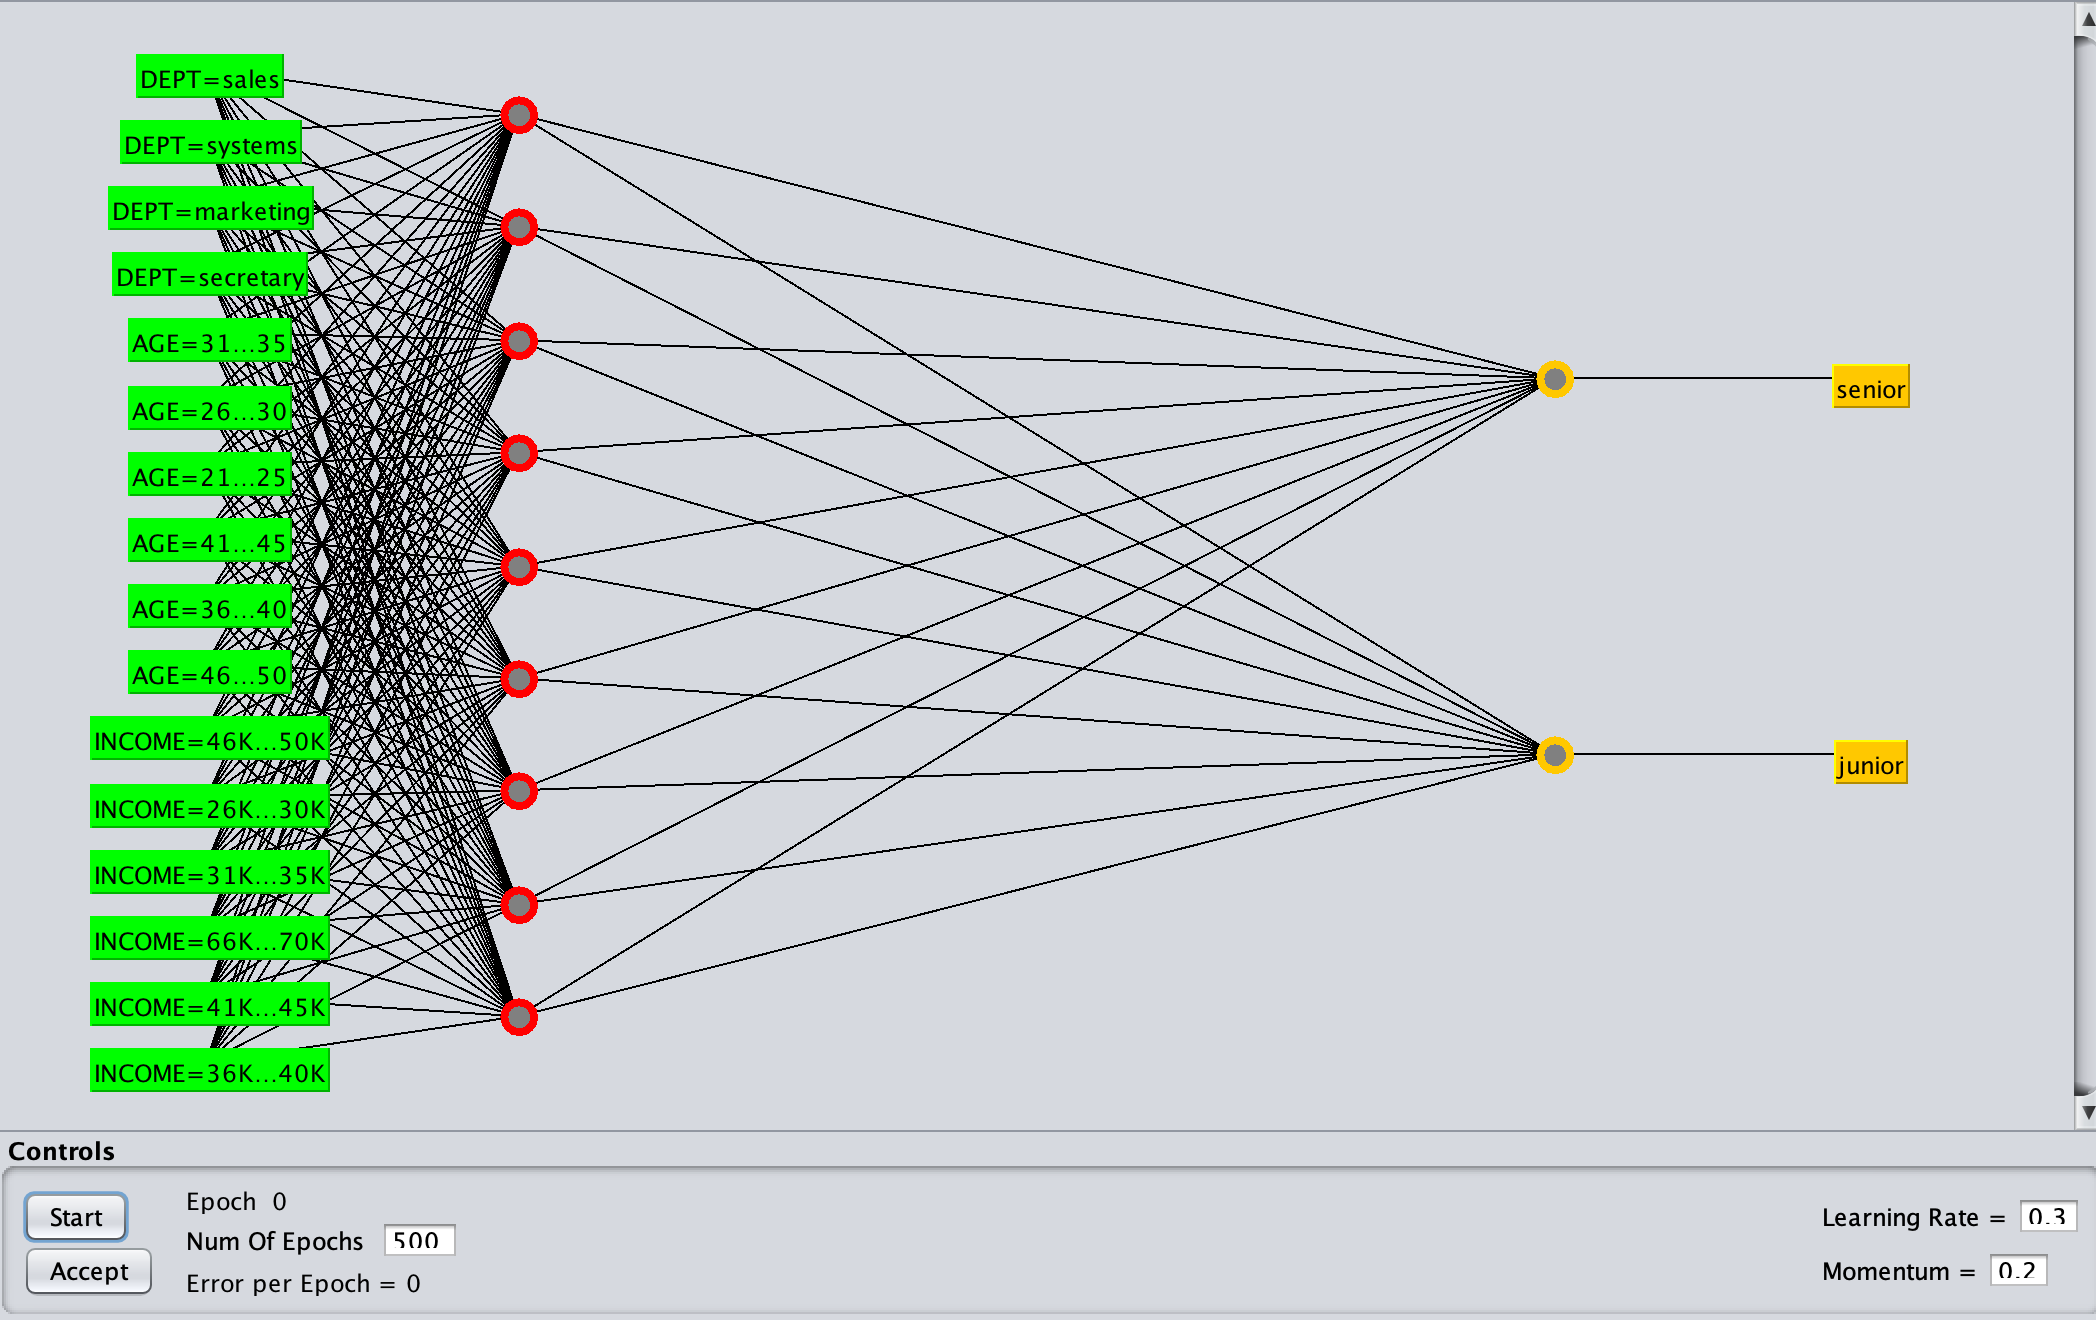
\includegraphics{mlp.png}
\caption{Multilayer Forward Feed Network}
\end{figure}

    \paragraph{(b) Using the multilayer feed-forward neural network obtained
in (a), show the weight values after one iteration of the back
propagation algorithm, given the training instance
``(sales,senior,31...35,46K...50K)''. Indicate your initial weight
values and biases and the learning rate
used.}\label{b-using-the-multilayer-feed-forward-neural-network-obtained-in-a-show-the-weight-values-after-one-iteration-of-the-back-propagation-algorithm-given-the-training-instance-salessenior31...3546k...50k.-indicate-your-initial-weight-values-and-biases-and-the-learning-rate-used.}

    Please see attached documents with output of Weka implementations of two
different classification models: SVM (results\_svm.pdf) and multilayer
feed forward neural network (results\_mlp.pdf).


    % Add a bibliography block to the postdoc
    
    
    
    \end{document}
